%! Author = adnansiddiquei
%! Date = 29/06/2024

% Preamble
\documentclass[a4paper,11pt]{article}
\pdfoutput=1

% Packages
%\usepackage[colorlinks=true, linkcolor=blue, urlcolor=blue, citecolor=blue, pdfborder={0 0 0}]{hyperref}
\usepackage{url}
\usepackage{jcappub}
\usepackage[T1]{fontenc}
\usepackage{listings}
\usepackage{roboto}
\usepackage{subcaption}
\usepackage{blindtext}
\usepackage{seqsplit}
\usepackage[nottoc]{tocbibind}
\usepackage{siunitx}
\DeclareSIUnit\angstrom{\text {Å}}

%\newcommand{\inlinecode}[1]{\lstinline{#1}}
%\newcommand{\inlinecode}[1]{\texttt{#1}}
\newcommand{\inlinecode}[1]{\texttt{\seqsplit{#1}}}
\lstset{basicstyle=\fontfamily{pcr}\selectfont}


\title{\boldmath Reproducing AstroCLIP: Executive Summary}

% %simple case: 2 authors, same institution
\author{Adnan Siddiquei}
\affiliation{University of Cambridge}

% e-mail addresses: one for each author, in the same order as the authors
\emailAdd{as3438@cam.ac.uk}
\note{Word Count: 905 (not including figure captions).}


\begin{document}
%    \abstract{}

\maketitle
\flushbottom

\section{Background and Motivation}\label{sec:introduction}
The size of scientific datasets, particularly in the field of astronomy, has been growing at an ever-increasing rate
over the last couple of decades.
Spectroscopic surveys such as the Sloan Digital Sky Survey (SDSS)\footnote{https://www.sdss.org/}~\citep{york2000} and
more recently the Dark Energy Spectroscopic Instrument (DESI)\footnote{https://www.desi.lbl.gov/} have been collating millions of
galaxy spectra over the last decade.
Similarly, photometric surveys such as the DESI Legacy Survey~\citep{desilegacy2018} has been imaging large portions
of the sky extracting millions of sources.
Both photometric and spectroscopic surveys are essential tools in modern astronomy and these datasets are used for
a variety of scientific purposes, from understanding the large scale structure of the universe;
estimating galaxy properties such as redshift, stellar mass, and star formation rate; to identifying rare objects such as
quasars and supernovae; and many more.
However, the growing data set size and diversity makes much of this difficult and traditional methods are often
limited by the quality of the data and its associated labels.
One such example is morphological classification, where we desire to classify galaxies into different types based on their
shape and structure, such as spiral or elliptical.
A decade ago we had crowdsourced campaigns such as Galaxy Zoo 2~\citep{willet2013} which classified approximately
300,000 galaxies, we now have tools such as Tractor\footnote{https://github.com/dstndstn/tractor}
which can probabilistically identify sources from photometric surveys and infer properties such as morphological classification.
More recently, given the unavailability of high quality labels, unsupervised and self-supervised learning methods have been
gaining popularity to tackle these sorts of tasks.
For example:
\begin{itemize}
    \item \cite{liang2023} train a 1D convolutional spectrum autoencoder on spectral data for the purposes of outlier
    detection;
    \item \cite{stein2021} train a 2D convolutional image embedder using a self-supervised technique on galaxy images
    for the purposes of similarity search;
    \item \cite{hayat2021} also use a self-supervised technique to train a 2D convolutional model to estimate distances to galaxies from their
    photometric images, and further demonstrate that the learned embeddings can be fine-tuned very effectively for redshift estimation;
\end{itemize}
~\cite{hayat2021} also show that significantly better performance can be acquired through fine-tuning the self-supervised
pre-trained model compared to simply training a supervised model from scratch.
This conclusion is not uncommon in the field of machine learning outside of astronomy and demonstrates the power
of transfer learning and the importance of foundation models for astronomical datasets.

However, as of yet most of these self-supervised learning methods have only been applied to a single modality despite
promising results in cross-modal contrastive learning outside of astronomy, such as contrastive language-image pre-training CLIP~\citep{radford2021}.
~\cite{astroclip} pioneer on this front by proposing a multi-modal contrastive learning approach to embed galaxy spectra
and galaxy images into a shared low-dimensional latent space, and in this paper we aim to reproduce their results.
Given the multi-modal nature of astronomical datasets, a useful astronomical foundation model should be able to embed
the varying views of the same object effectively into a shared latent space, allowing for in-modal and cross-modal downstream
application through zero-shot or few-shot learning.

\section{A Review of AstroCLIP}\label{sec:original-paper}
\cite{astroclip} present AstroCLIP, a cross-modal foundation model for galaxies.
Their approach consisted of two main components.
They first pre-train a novel transformer-based spectrum embedder on spectroscopic data from the DESI Early Data Release~\citep{desiearly2023}
through a self-supervised mask filling technique; and pre-train a vision transformer~\citep{dosovitskiy2021} image embedder
on galaxy images from the DESI Legacy Survey~\citep{desilegacy2018} using the DINO v2 self-supervised learning framework~\citep{oquab2024}.
Following this, they fine-tune the two embedders under the InfoNCE loss~\citep{oord2019} to align the embeddings
into a shared 512-dimensional latent space, the same pre-training datasets are used.
They demonstrate that the embeddings are well-aligned by using the embeddings to perform a variety of downstream zero-shot
and few-shot tasks, including in-modal and cross-modal similarity search, redshift prediction, and galaxy property prediction.

\section{Reproduction}\label{sec:reproduction}
\begin{figure}[t]
    \centering
    \makebox[\textwidth]{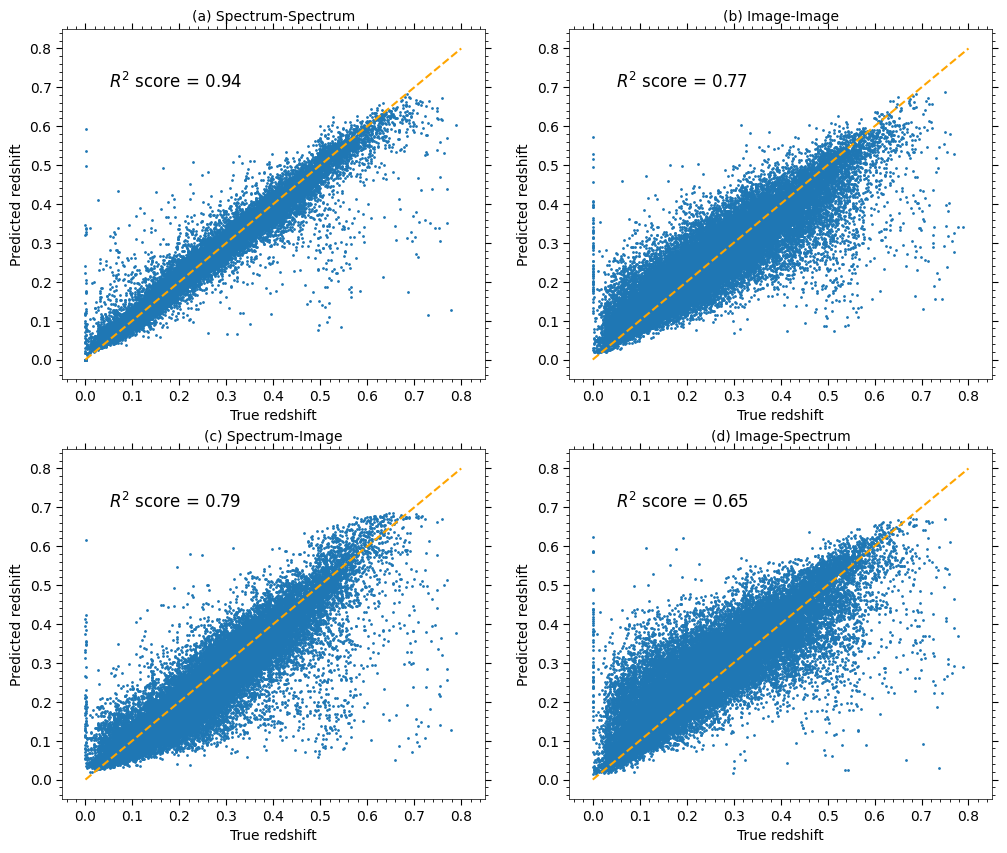
\includegraphics[width=1\textwidth]{figures/redshift_knn_regression}}
    \caption{In-modal and cross-modal zero-shot redshift predictions using k-NN regression on the learned embeddings for the
    best 128-dimensional embedding model.
    The y-axis shows the predicted redshift (the average of the 16 closest neighbours in terms of Euclidean distance) and the x-axis shows the true redshift.
    The dashed line represents a perfect prediction, and the $R^{2}$ of the fit is shown in the top left corner.
    $S_{kNN}(\mathbf{z}_{q}^{sp}, \mathbf{z}^{im})$ indicates the cross-modal prediction where a spectrums redshift was
    predicted using its 16 closest embeddings derived from galaxy images.}
    \label{fig:rkr}
\end{figure}

\begin{figure}[t]
    \centering
    \makebox[\textwidth]{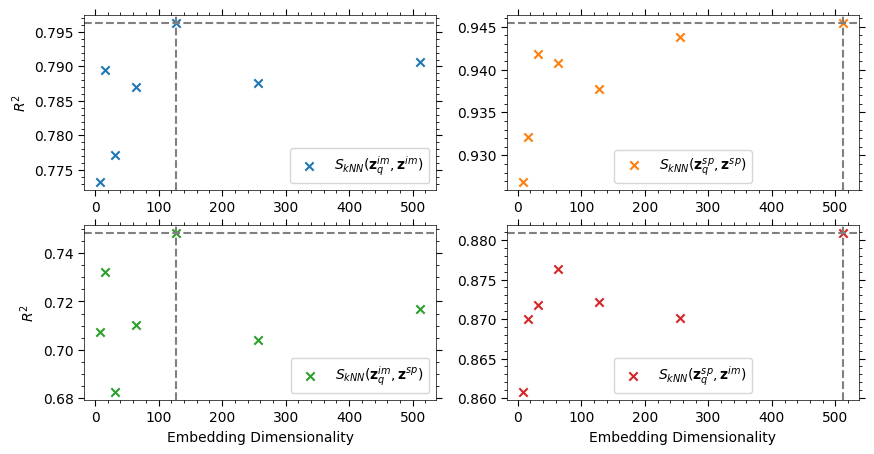
\includegraphics[width=1\textwidth]{figures/r2_vs_embedding_dim}}
    \caption{Exactly the same results as shown in Figure~\eqref{fig:rkr}, but plotted more succinctly for all embedding
    dimensionalities, and all types of in-modal and cross-modal prediction types.
    Each plot shows a prediction type (corresponding to one of the 4 plots in Figure~\eqref{fig:rkr}).
    The x-axis is the embedding dimensionality and the y-axis is the $R^{2}$ value of the predictions.
    There are exactly 7 points on each plot, one for each embedding dimensionality tested.
    The dashed lines show the best model for each prediction type.}
    \label{fig:r2_vs_embedding_dim}
\end{figure}

\begin{figure}[t]
    \centering
    \makebox[\textwidth]{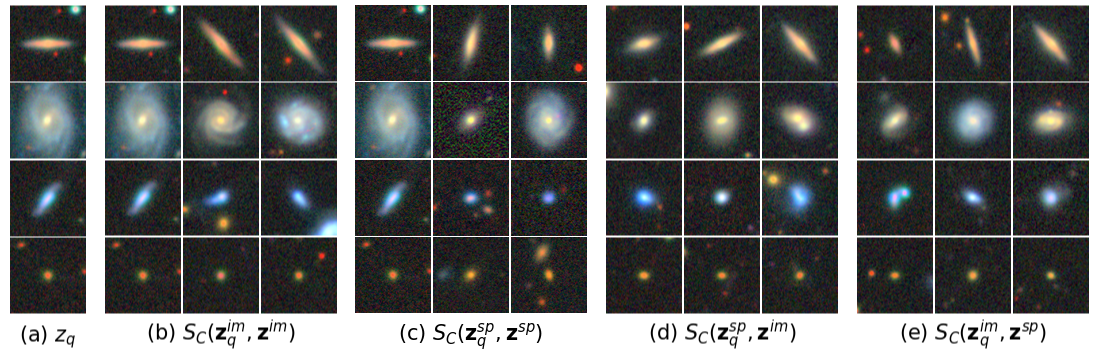
\includegraphics[width=1\textwidth]{figures/sim_search_images_all}}
    \caption{In-modal and cross-modal similarity search using cosine similarity on the learned embeddings for the
        best 128-dimensional embedding model.
        (a) shows the query galaxies; (b) shows the 3 most similar galaxies using an in-modal image to image search; and
        so on.
        By construction, the most similar in-modal galaxy to any given galaxy is itself, hence, the first column of images
        in (b) and (c) are identical to the query image in (a).}
    \label{fig:ssia}
\end{figure}

\begin{figure}[t]
    \centering
    \makebox[\textwidth]{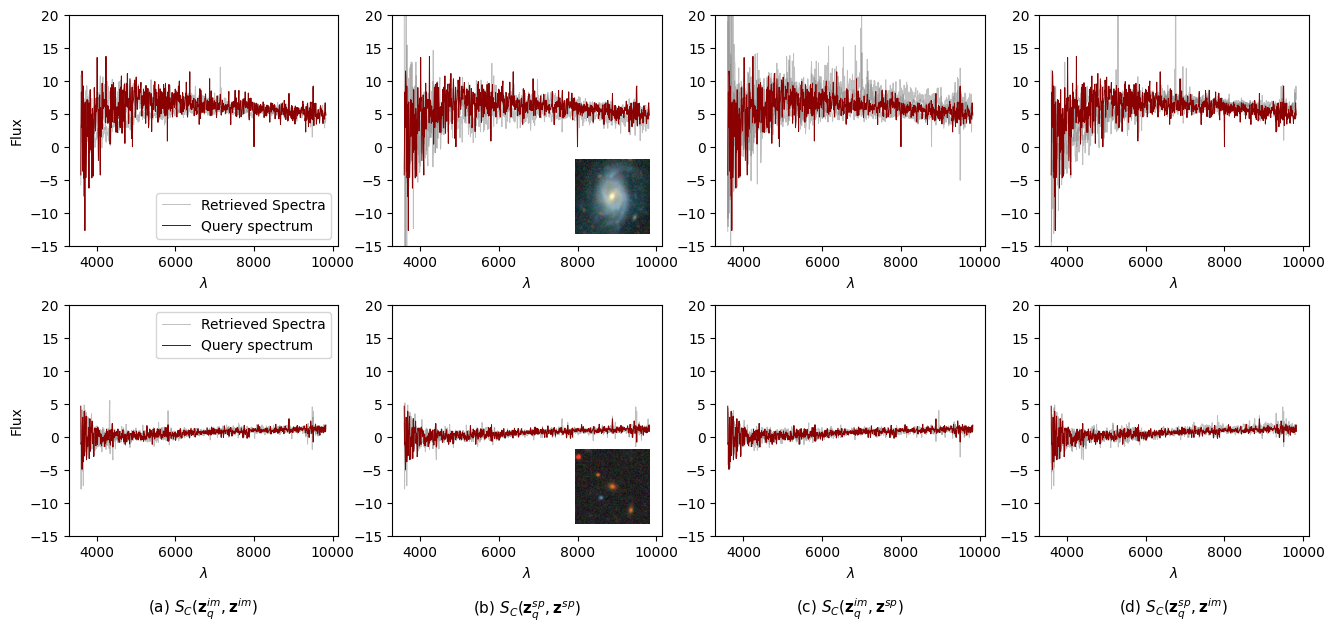
\includegraphics[width=1\textwidth]{figures/sim_search_spectra}}
    \caption{In-modal and cross-modal similarity search using cosine similarity on the learned embeddings for the
        best 128-dimensional embedding model.
        Each row in this figure depicts a single query galaxy (query spectrum in red, galaxy imaged in plot (b)), with
        each subfigure showing the spectrum of the 3 most cosine similar galaxies to the
        query galaxy by in-modal and cross-modal similarity search.}
    \label{fig:sss}
\end{figure}

We reproduce the AstroCLIP model, however we utilise the pre-trained convolutional spectrum embedder by ~\cite{liang2023}
and the pre-trained convolutional image embedder by ~\cite{stein2021} rather than pre-training our own.
We use the dataset as provided by ~\cite{astroclip}, and a variety of general and astronomy specific data augmentations
to increase the variety of the dataset.
In addition to the 512-dimensional model, we also train AstroCLIP variations to embed the spectra and images into
a variety of lower-dimensional latent spaces: $[8, 16, 32, 64, 128, 256]$.
We train each of these 7 models for 75 epochs, and choose the model with the lowest validation loss for analysis.

We assess the performance of our models using a subset of the downstream tasks presented in the original paper, specifically
zero-shot k-NN redshift estimation and retrieval by cosine similarity, these results are displayed in Figures~\eqref{fig:rkr},
~\eqref{fig:r2_vs_embedding_dim}, ~\eqref{fig:ssia}, and ~\eqref{fig:sss}.
Generally, we find equivalent performance in our reproduction.
We outperform their 512-dimensional model in the photometric redshift prediction task with our 128-dimensional
model achieving an $R^{2}$ value of 0.80 (Figure (\ref{fig:rkr}b)) compared to their 0.79; but fall short in the spectroscopic
redshift prediction task with an $R^{2}$ value of 0.94 (Figure (\ref{fig:rkr}a)) compared to their 0.98.

\section{Significance of Results}\label{sec:conclusion}
Our results alongside those of~\cite{astroclip} demonstrate that it is possible to achieve high quality foundation
models for astronomical data using cross-modal contrastive pre-training, and that the learned embeddings can be used for a variety
of downstream tasks with strong performance.
This has a variety of impacts on the field of astronomy, such as enabling cross-modal similarity searches for rare or interesting
objects, and enabling the use of pre-trained foundation models for transfer learning on smaller datasets for specific tasks,
thereby reducing the requirement for large amounts of high quality labels.


\clearpage

%\nocite{*}
\bibliographystyle{apalike}
\bibliography{exec-summary}
\clearpage

%\appendix

%\section{Appendix A}\label{app:app-a}
%Lorem ipsum dolor sit amet, consectetur adipiscing elit. Suspendisse eget urna laoreet, elementum tellus nec, dapibus dui.
\end{document}
